\section{Application Categorization}\label{sec:appl}

\if 0
\begin{figure*}[htp]
  \begin{center}
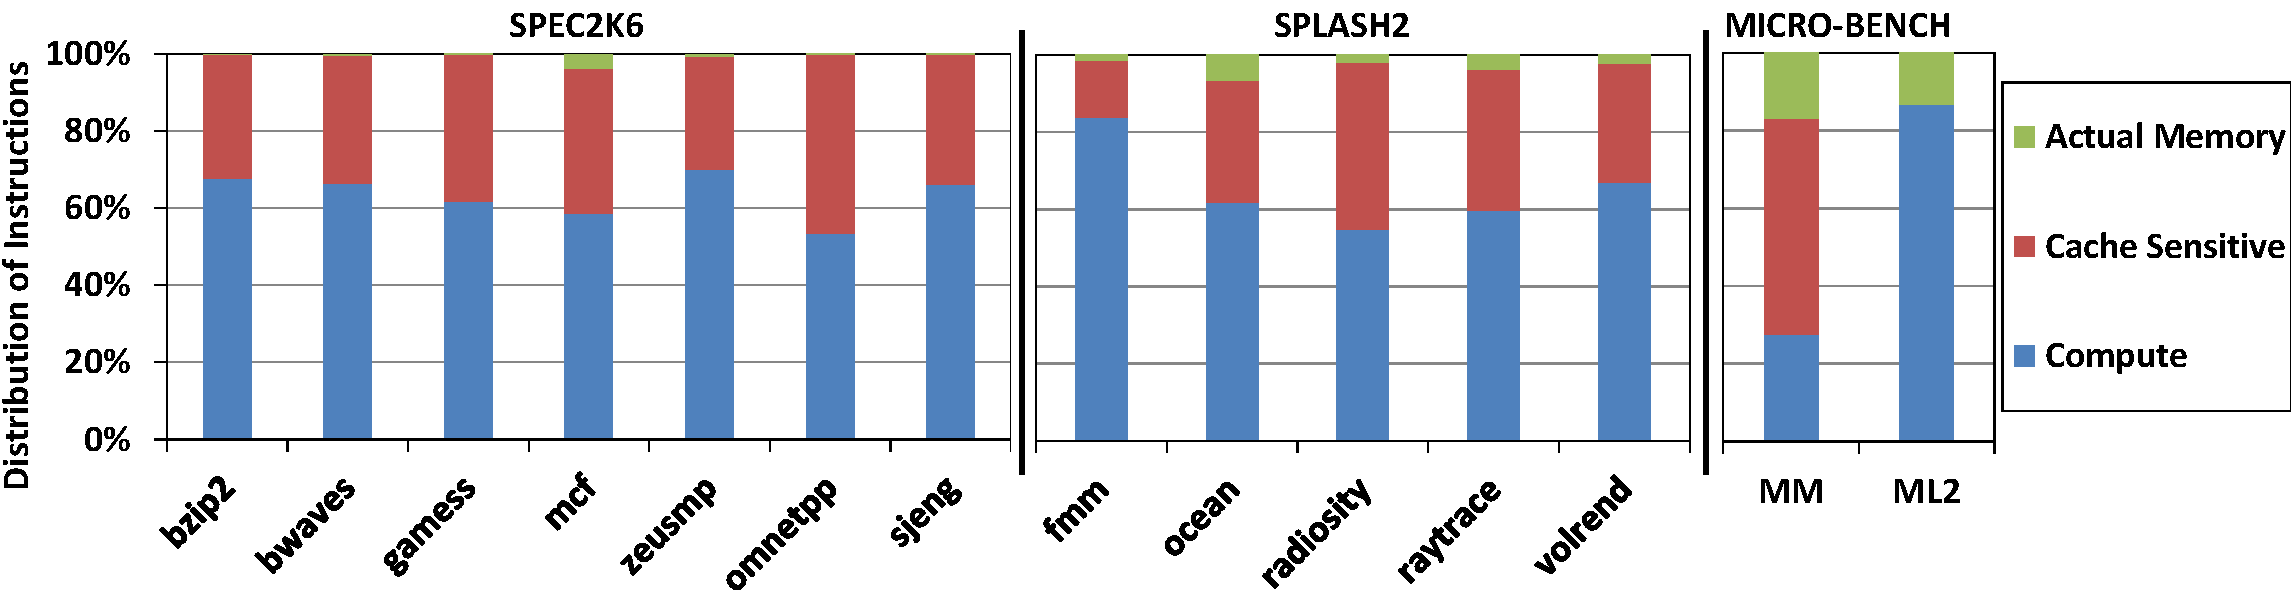
\includegraphics[width=\linewidth]{figs/app-cat-crop.pdf}
  \end{center}
  \vspace{-0.1in}
  \caption{Application Categorization}
  \label{fig:def-perf}
\end{figure*}
\fi

To first analyze the applications and profile them , we used PIN~\cite{pin} binary instrumentation tool. The PIN tool was modeled to account for total instructions in the application, instructions which get hit in the cache and instructions which actually access memory. 
This profiling was done mainly to account for
which frequency to scale (CPU or DRAM) based on the application information. 
We did not model the Disk (I/O) instructions, as PIN cannot model file system accesses, and
we have no control over the speed at which DISK accesses happen. So, our focus is
mainly on 3 categories:

\begin{itemize} 
\item \textit{Compute Intensive}: The application which spend their time in CPU core and have
more instructions between load/stores to memory. For these applications, CPU
frequency is the important parameter.
\item \textit{Cache Sensitive}: The applications which have more memory access instructions,
but due to the locality of the data accesses, most of them get the data in CPU caches.
For these applications, again CPU frequency is important. It is possible that just
profiling the memory related instructions could be misleading as you do not want to
scale DRAM frequency for cache-sensitive applications.
\item \textit{Memory Bound} These are the applications, which have lot of cache misses
and the accesses reach memory. Increasing CPU frequency for these applications could 
lead to wastage of energy. 
\end{itemize}

Figure~\ref{fig:app-cat} shows the application categorization across 7 SPEC2006~\cite{spec2006} benchmarks, 5 SPLASH2~\cite{splash2} benchmarks and 2 micro-benchmarks. 
It is clear that SPEC2006 benchmarks are mostly compute intensive, 
SPLASH2 workloads are Compute and cache sensitive, whereas the 2 micro-benchmarks 
have lot of memory accesses.

\if 0
\begin{figure*}[ht]
  \begin{center}
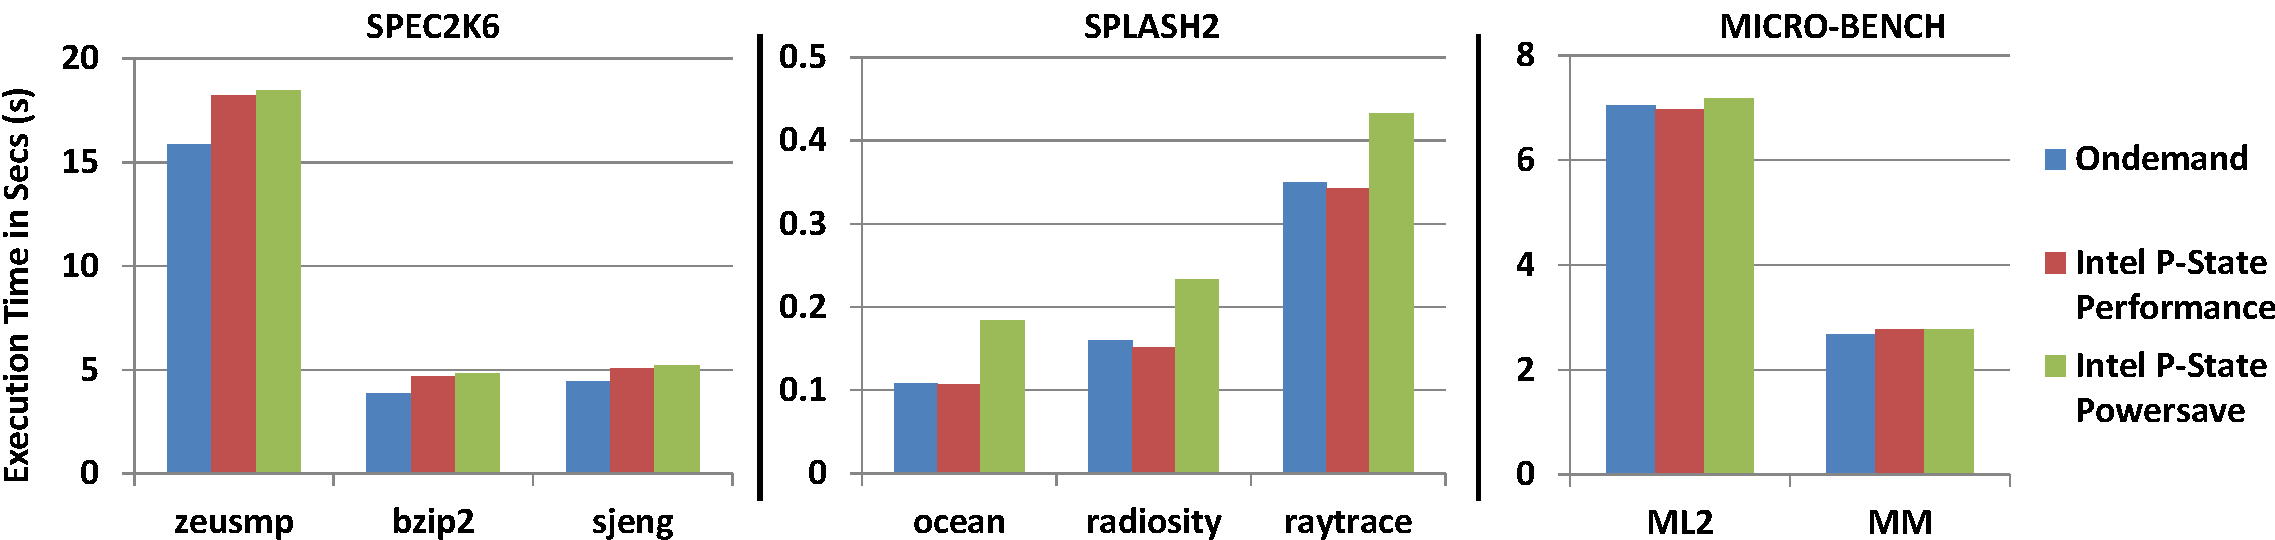
\includegraphics[width=\linewidth]{figs/def-exec-time-crop.pdf}
  \end{center}
  \vspace{-0.1in}
  \caption{Execution time for Linux Ondemand and Intel-Pstate power governors}
  \label{fig:def-perf}
\end{figure*}
\fi

Now, we analyzed these workloads with Linux "Ondemand" power governor and 2 power governors of recent Intel P-state driver~\cite{pstate}. Figure~\ref{fig:def-perf}
shows the execution time of chosen workloads for the three power governors. It is seen that, even though each of the power governors
have distinct objectives they all perform similar. TO check, whether it was same with
energy efficiency of these governors, we performed energy evaluation for all 3 application categories.


\if 0
\begin{figure}[h]
  \begin{center}
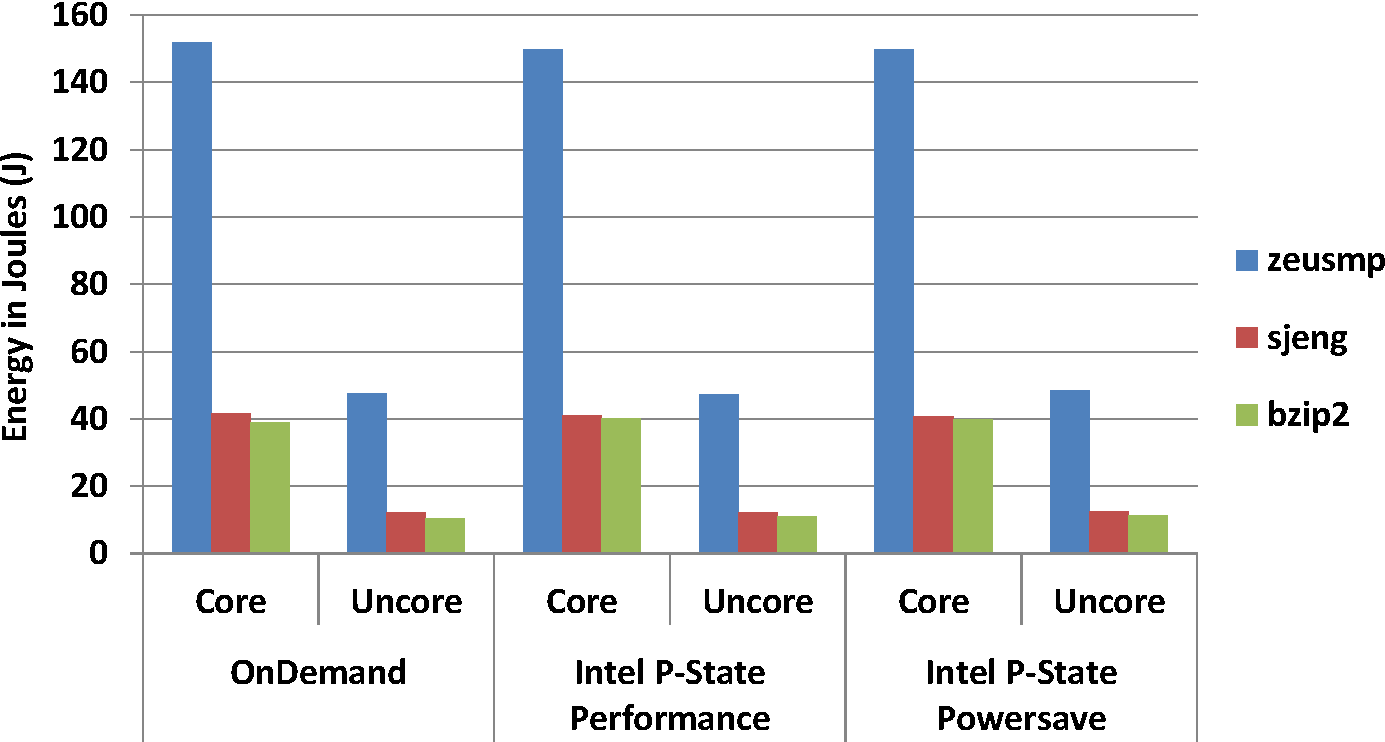
\includegraphics[width=\linewidth]{figs/def-drivers-spec-crop.pdf}
  \end{center}
  \vspace{-0.1in}
  \caption{Energy Consumption for SPEC2006 workloads}
  \label{fig:spec-energy}
\end{figure}
\fi

\if 0
\begin{figure}
  \begin{center}
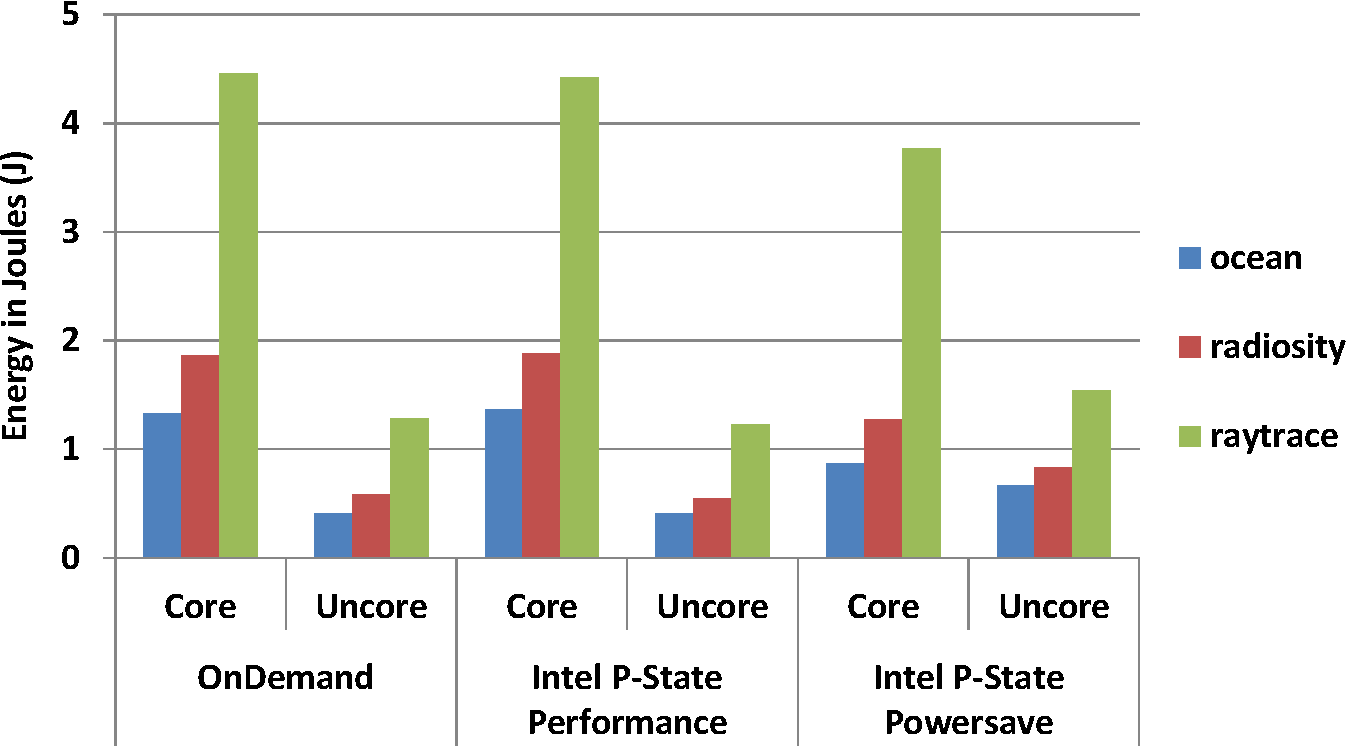
\includegraphics[width=\linewidth]{figs/def-drivers-splash-crop.pdf}
  \end{center}
  \vspace{-0.1in}
  \caption{Energy Consumption for SPLASH2 workloads}
  \label{fig:splash-energy}
\end{figure}
\fi

\if 0
\begin{figure}[h]
  \begin{center}
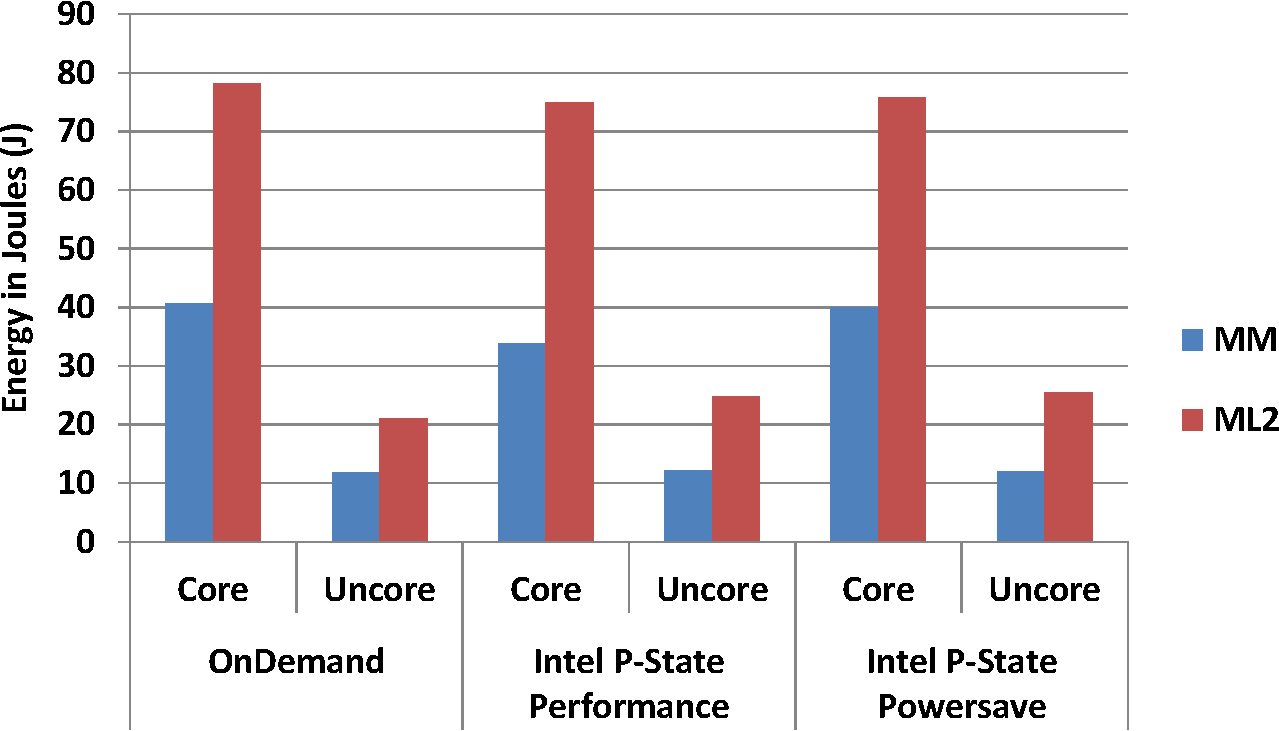
\includegraphics[width=\linewidth]{figs/def-drivers-micro-crop.pdf}
  \end{center}
  \vspace{-0.1in}
  \caption{Energy Consumption for Micro-benchmarks}
	\label{fig:micro-energy}
\end{figure}
\fi

Figure~\ref{fig:spec-energy} shows the energy consumption in Joules for 3 of the SPEC 2006
benchmarks and we see that the Core and Uncore energy for all 3 workloads with 3 different
power governors are similar. 
Figure~\ref{fig:splash-energy} shows similar trend for SPLASH benchmarks,
but for all 3 workloads it is seen that with Psate powersave governors we get some energy benefits.
This slight benefit is because of some memory access these benchmarks have and powersave governor
gains energy benefits by reducing the CPU frequency to minimum. 
Figure~\ref{fig:micro-energy} shows
the energy consumption for 2 of the memory bound micro-benchmarks and again similar trend is seen
for all the 3 governors.

The takeaway for these analysis is that, existing linux power governors randomly
choose a frequency range and dynamically switch based on the system load
without considering the application property. We next, show that how 
application information can be used to make better policy decisions and 
save energy.



